% !TEX encoding = UTF-8 Unicode
%!TEX TS-program = xelatex

\documentclass[12pt]{extarticle}
% extarticle is like article but can handle 8pt, 9pt, 10pt, 11pt, 12pt, 14pt, 17pt, and 20pt text

\def \ititle {Origins of Mind}
 
\def \isubtitle {Lecture 08}
 
\def \iauthor {Stephen A. Butterfill}
\def \iemail{s.butterfill@warwick.ac.uk}
\date{}

%for strikethrough
\usepackage[normalem]{ulem}

\usepackage{pdfpages}


\input{$HOME/Documents/submissions/preamble_steve_handout}

%logic symbol \leftmodels
\usepackage{MnSymbol}

%\bibpunct{}{}{,}{s}{}{,}  %use superscript TICS style bib
%remove hanging indent for TICS style bib
%TODO doesnt work
\setlength{\bibhang}{0em}
%\setlength{\bibsep}{0.5em}


%itemize bullet should be dash
\renewcommand{\labelitemi}{$-$}

\begin{document}

%\raggedcolumns

\begin{multicols*}{3}

\setlength\footnotesep{1em}


\bibliographystyle{newapa} %apalike

%\maketitle
%\tableofcontents




%--------------- 
%--- start paste
\def \ititle {Logic (PH133)}
 
\def \isubtitle {Lecture 7}
 
\begin{center}
 
{\Large
 
\textbf{\ititle}: \isubtitle
 
}
 
 
 
\iemail %
 
\end{center}
 
Readings refer to sections of the course textbook, \emph{Language, Proof and Logic}.
 
 
 
 
 
 
\section{Something Is Above Something}
 
\emph{Reading:} §11.1
 
\begin{minipage}{\columnwidth}
 
Something is above something:
 
\hspace{3mm} ∃x ∃y Above(x,y)
 
\end{minipage}
 
 
 
\section{There Is Exactly One}
 
There is one creator (at least one, maybe more).
 
\hspace{3mm} ∃x Creator(x)
 
Ahura Mazda is the one and only creator.
 
\hspace{3mm} Creator(a) ∧ ∀x( Creator(x) → x=a )
 
All squares are broken.
 
\hspace{3mm} ∀x( Sqr(x) → Brkn(x) )
 
There is one and only one creator.
 
\hspace{3mm} ∃y( Creator(y) ∧ ∀x( Creator(x) → x=y ) )
 
\hspace{3mm} or:
 
\hspace{3mm} ∃y ∀x( Creator(x) ↔ x=y )
 
 \columnbreak
 
 
\section{∃Intro}
 
\emph{Reading:} §13.2
 
\begin{center}
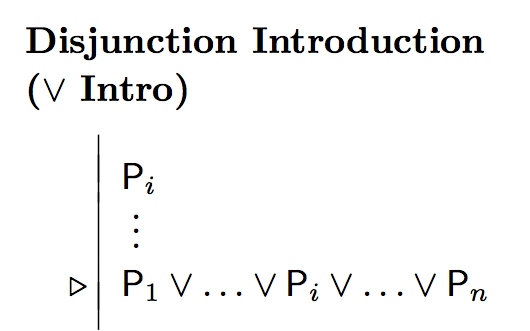
\includegraphics[scale=0.3]{img/rule_disjunction_intro.png}
\end{center}
 
 
\section{∃Elim}
 
\emph{Reading:} §12.2, §13.2
 
\begin{center}
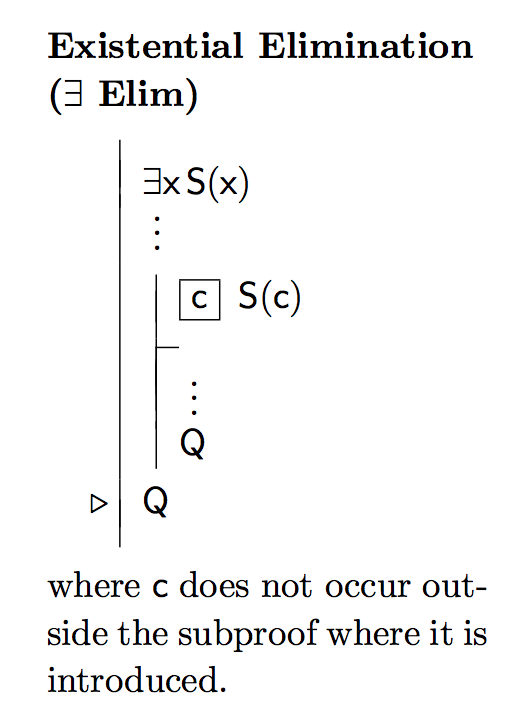
\includegraphics[scale=0.3]{img/rule_existential_elim.png}
\end{center}
\begin{center}
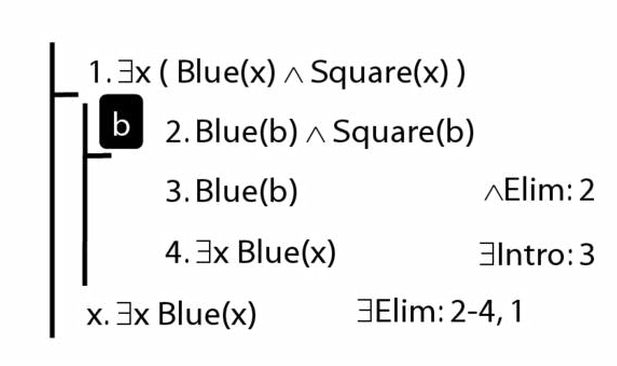
\includegraphics[scale=0.3]{img/proof_existential_elim.png}
\end{center}
\begin{minipage}{\columnwidth}
 
Note this restriction on the use of ∃Elim:
 
\begin{center}
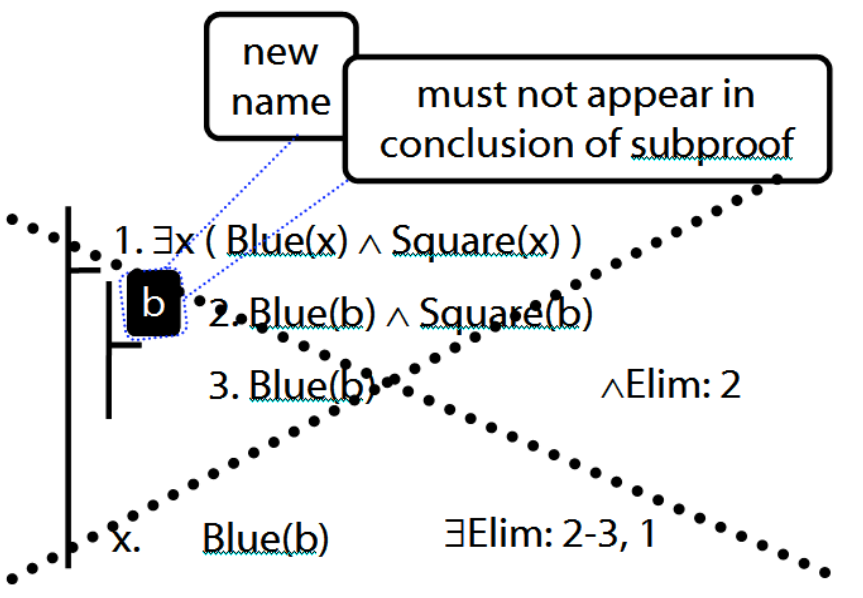
\includegraphics[scale=0.3]{img/proof_existential_elim_incorrect.png}
\end{center}
\end{minipage}
 
 
 
\section{Translation with Quantifiers}
 
\emph{Reading:} §9.5, §9.6
 
\begin{minipage}{\columnwidth}
 
All discordians weep:
 
∀x( Dscrdn(x) → Wps(x) )
 
\end{minipage}
 
\begin{minipage}{\columnwidth}
 
All \textbf{French} discordians weep:
 
∀x( ( \textbf{Frnch(x) ∧} Dscrdn(x) ) → Wps(x) )
 
\end{minipage}
 
\begin{minipage}{\columnwidth}
 
All French discordians weep \textbf{and wail}:
 
∀x( ( Frnch(x) ∧ Dscrdn(x) ) → ( Wps(x) \textbf{ ∧ Wls(x)} ) )
 
\end{minipage}
 
\begin{minipage}{\columnwidth}
 
All French discordians weep and wail \textbf{except Gillian Deleude}:
 
∀x( ( Frnch(x) ∧ Dscrdn(x) \textbf{∧ ¬(x=a)} ) → ( Wps(x) ∧ Wls(x) ) )
 
\end{minipage}
 
 
 
\section{Scope and Quantifiers}
 
\emph{Reading:} §9.5, §9.6
 
\begin{minipage}{\columnwidth}
 
Underlining shows the scope of the quantifiers:
 
\begin{center}
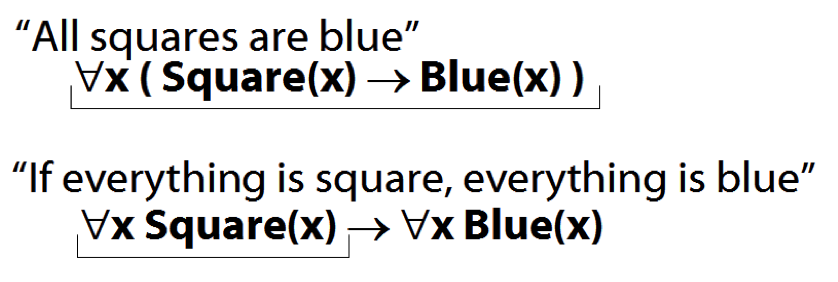
\includegraphics[scale=0.23]{img/scope_quantifiers.png}
\end{center}
\end{minipage}
 
 
 
\section{∀Intro}
 
\emph{Reading:} §12.1, §12.3, §13.1
 
\begin{center}
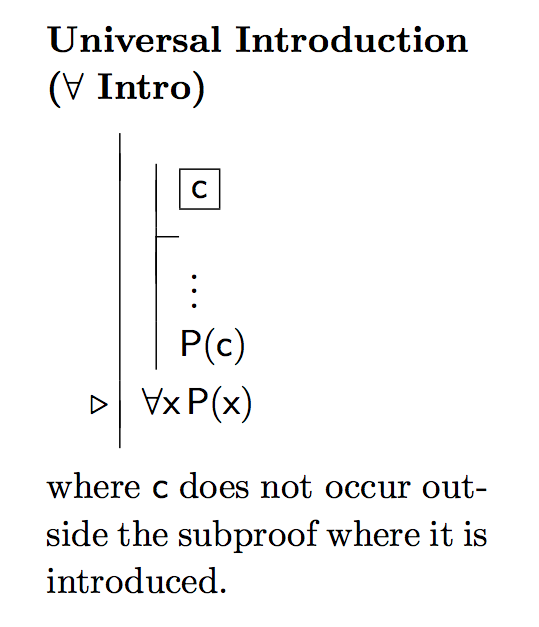
\includegraphics[scale=0.23]{img/rule_universal_intro.png}
\end{center}
\begin{center}
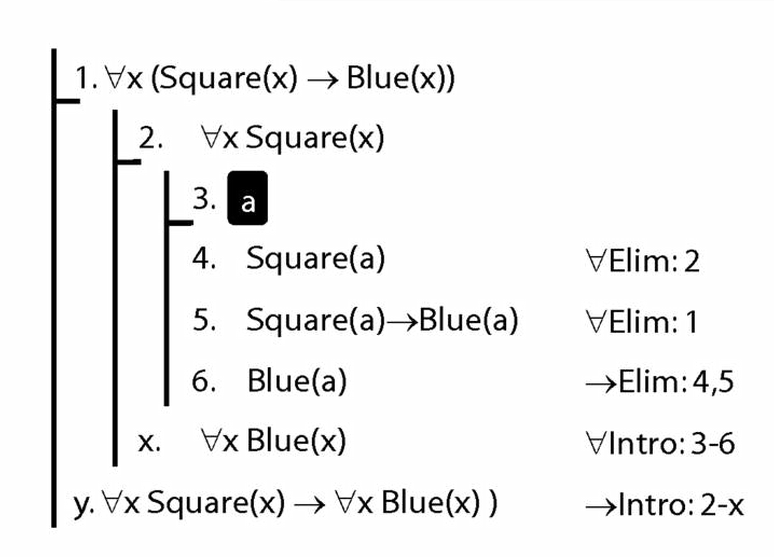
\includegraphics[scale=0.3]{img/proof_universal_intro.png}
\end{center}
\begin{minipage}{\columnwidth}
 
\

\

\
 
Why is this proof incorrect?
 
\begin{center}
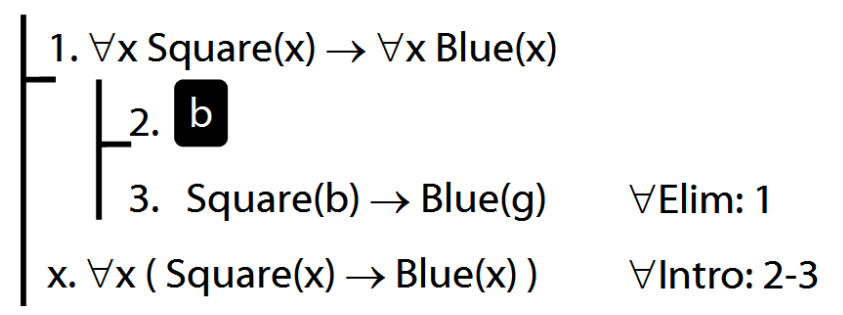
\includegraphics[scale=0.3]{img/proof_universal_intro_incorrect.png}
\end{center}
\end{minipage}
 
 \vfill
\columnbreak
\section{Summary of Quantifier Rules}
 
\emph{Reading:} §13.1, §13.2
 
\begin{center}
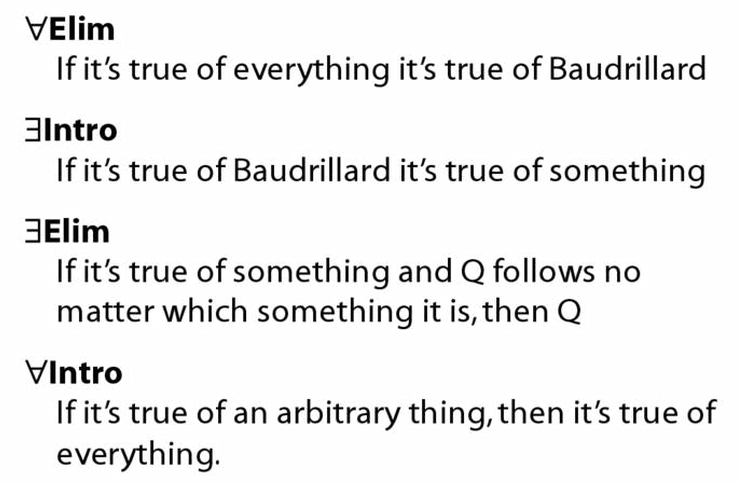
\includegraphics[scale=0.3]{img/quantifier_rule_summary.png}
\end{center}
 
 
\section{Two Things Are Broken}
 
\emph{Reading:} §14.1
 
To translate sentences involving number into FOL, use identity. For example,
 
`Two things are broken' might be translated as:
 
∃x ∃y ( Broken(x) ∧ Broken(y) ∧ ¬(x=y) )
 
\vfill

%--- end paste
%--------------- 
 


\end{multicols*}

\end{document}